\chapter{System Architecture}
\label{chap:System Architecture}

% 6 pages
The main goal of this work is to compare different interpolation techniques that are based on traditonal (statistical) and ML-based approaches. ML-based approaches first of all need a lot of data to be trained and validated with, and after deployment need access to relevent real-time data, if near real-time capabilities are desired. In the context of smart city, such ML-based interpolation models could be used to improve data availibility by interpolating missing/unavailable data such as LST readings under cloudy conditions, and be incoperated into a service that other services, like a UHI detection service, could further rely on, without the need to implement interpolation techniques themselves. This could reduce costs to develop such depending services, as they no longer need to deal with missing data themselves while also improving interpolation results with well-trained and designed models.

\begin{figure}[h]
    \centering
    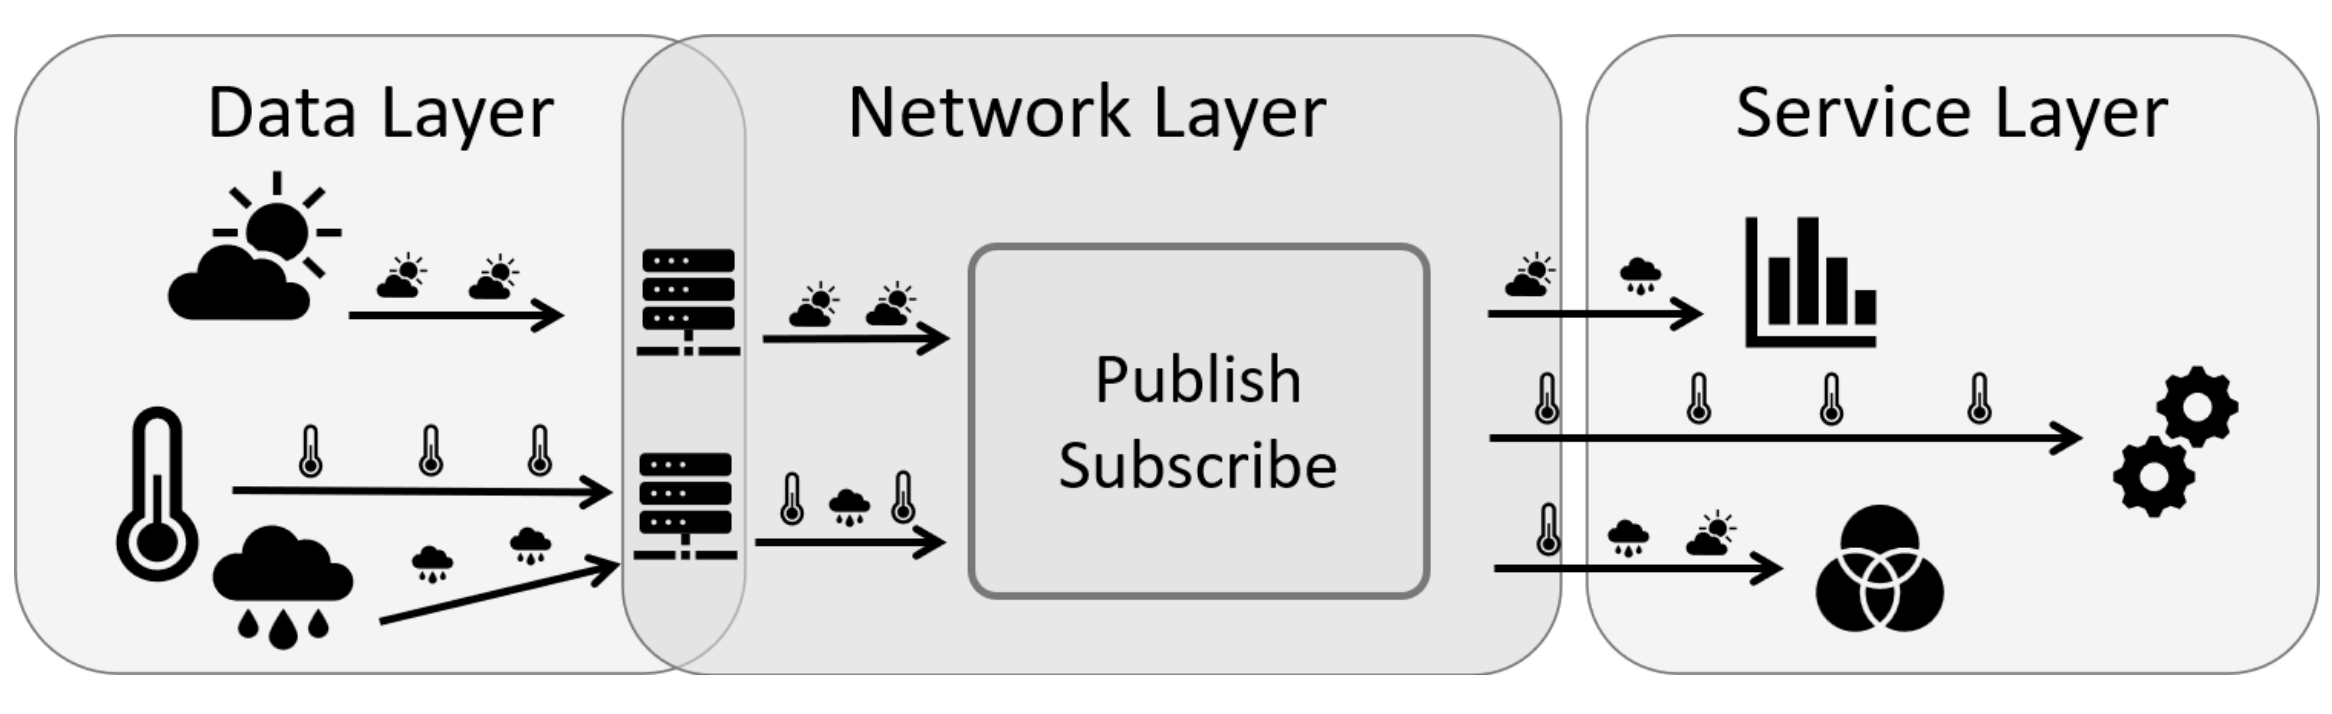
\includegraphics[width=\textwidth]{images/expose-system-architecture.png}
    \caption{In the data layer (left), a wide variety of environmental data is collected with the help of multiple sensors. These are connected to their citizen-owned local base stations, which manage access rights and forward collected data to subscribed services (right) via the decentralized publish-subscribe in the network layer (center).}
    \label{fig:system-architecture-overview} %todo: create graphic of the 4 layers instead
\end{figure}

First, we need to take a look at how such a service fits into existing smart city architectures. The most generalised architecture of a smart city consists of four layer, the sensing layer, transmission layer, data management, and application layer~\cite{silva2018towards}. In this work, we focus on the sensing layer, dealing with topics such as correct sensor placement and underlying footprint, and the application layer, which accesses available data via data management services to provide additional services to the city and its citizens. For the data transmission and data management layers, there already are different technologies and service offerings, that aim at solving the underlying problems, e.g. network bandwidth, network availability, sensor discoverability, handling the massive amounts of data that is already or will be collected in the future, and many more. For the communication and discovery of sensor nodes, one solution could be SkipNet~\cite{harvey2002skipnet}, an overlay network focused on discoverability while also protecting privacy, with which the data transportation layer could be desinged as a peer-to-peer (P2P) network. Other research focuses on the data accessability and discoverability, by making data accessible for everyone, not only for economic partners in a closed-off system. Examples would be the Smart Networks For Urban Citizen Participation (SANE) initiative~\cite{bornholdt2019sane}, which... Figure \ref{fig:system-architecture-overview} shows the architecture of the SANE system.

\section{Sensing Layer}

% todo: take a closer look at sensing layer with challenges like sensor placement, uncertainty etc.

The goal for the sensing layer is to monitor the surrounding environment and capture key data for further analysis and decision making. It consists of many different types of physical and virtual sensors. The first group of sensors are the physical sensors, which are placed directly inside the environment. Wireless sensor networks (WSN) have seen a lot of attention for many different applications such as `military sensing, physical security, air traffic control, traffic surveillance, video surveillance, industrial and manufacturing automation, distributed robotics, environment monitoring, and building and structures monitoring'~\cite{chong2003sensor}. The challenges for WSNs primarily depend among other things on the deployment. An ad-hoc WSN has energy and bandwidth contraints due to the usage of batteries as power sources.
In Contrast, sensors that are permanetly installed, either stationary or on a moving target, and connected to a constant power source don't have this constraints. This approach could be used for smart cities to reduce waste and guarantee representative measurements via correct sensor placement. In the case of stationary sensor networks though, the initial deployment and following maintenance cost can be substantial~\cite{chapman2015birmingham}.\\
In recent years, low-cost sensors (LCS) in combination with sensor networks have enabled fine-granular real-time monitoring of urban environments, although the quality of individual low-cost sensors can be questionable~\cite{castell2017can}. In general, LCSs can improve data availibility and support analysis, but do not substitute well-calibrated reference instrumentation~\cite{lewis2018low}.
% could also discuss low cost sensors

\subsection{Stationary Sensor Types}
There are many different types of environmental features that can be measured directly inside an urban area. The types of measurements that can be observed are among others: air temperature, humidity, atmospheric pressure, reactive gaseous air pollutant (CO, NOx, O$_3$, SO$_2$), particulate matter (PM), greenhouse gases (CO$_2$, CH$_4$), percipitation, solar radiation, wind speed and direction, anthropogenic heat, noise, sky-view factor, heat fluxes and many more. Correlations between these features can vary greatly based on surrounding factors. In order to better understand these correlations, many empirical studies have studied the influence of meteological factors on features such as PM~\cite{tai2010correlations}. Additionally, many fields of statistics have specialised on topics such as statistics in climatology~\cite{von2002statistical}, geostatistics~\cite{trangmar1986application} and more.\\
All sensor readings that are taken by physical sensors are singular data points. Additionally to the type of measurement taken and the actual value observed, physical sensor readings include the physical location of the sensor, e.g. latitude, longitude and altitude, the type of sensor used to take the measurement, and the sampling rate. For air temperature, the sampling rate could be an average temperature measured over five minutes, whereas percipitation might be measured by collecting rain for certain periods of time and then measuring the amount of rain collected. The sensor type is important, as different types of sensors can produce different qualities of measurements, e.g. LCS compared to callibrated reference-grade high cost sensors, and perform better or worse based on the meteological conditions, e.g. worse performance at low temperatures, high humidity etc. Due to the placement directly inside the environment, (near) real-time observation and high temporal resolution are generelly possible, but might be infleunced by network availability etc. The spatial resolution highly depends on the number of sensors deployed and the correct placement of the sensors. The correct placement has a direct influence on the footprint of the sensor~\cite{leclerc2014footprints} and the representativness of the measurement taken for the underlying and surrounding area~\cite{oke2006guideline}.

% need to be exchanged more often due to environmental influences

% Todo: list of sensors with downsides

\subsection{Remote Sensing}
% remote sensing

In comparison to stationary sensors that are installed directly in the environment they are observing, remote sensing describes the process of observing a target environment from afar~\cite{campbell2011introduction}. In climatology, remote sensing is used to collect meteological data via satellites, planes or ballons by either capturing image data, that can be used to identify things like cloud and land coverage, by measuring passive radiation, or by actively sending out microwaves or using LIDAR to detect features such as surface temperature, e.g. LST data. Remote sensing comes with its own set of challenges.

% remote sensing challenges

- 





- sensing layer: (wireless) sensor networks, virtual sensors via APIs/middlewares, sensors as database (bad), privacy

- overview types of sensors, challenges for each
- discussion premium vs low-cost sensors
- discussion static data incorporation -> NDVI from geoportal via data management layer

- P2,5: highly depends on air flows
- humidity: needs to be replaced more often due to pollution
- temperature

- modelling of the sensing layer in this thesis: collect actual data (maybe lack of sensor descriptions), simulation (but very complex weather models)

% rest
- overview of remote sensing sensor types and downsides (clouds etc.)

- discussion virtual sensors/static content

% todo

The \textit{sensing layer} consists of many different data sources. In the context of temperature sensing and prediction, this could include single (inexpensive) sensors such as the popular BMP280 \footnote{https://www.bosch-sensortec.com/products/environmental-sensors/pressure-sensors/bmp280/}, private weather stations such as sold by Netatmo \footnote{https://www.netatmo.com/en-gb/weather/weatherstation} hidden behind an API \footnote{https://dev.netatmo.com/apidocumentation/general}, public weather station data such as from the Deutscher Wetterdienst (DWD) \footnote{https://www.dwd.de/} which offer an API and historic weather data, or other geologically relevant data such as zoning plans which, in the case of the city of Hamburg in Germany, can be accessed via an OpenData platform provided by the State Office for Geoinformation and Surveying Hamburg \footnote{https://geoportal-hamburg.de/geo-online/}. In order to gain detailed insights into urban microclimates, we need fine-grained spatial and temporal data. As managing and maintaining such a large sensor network as a single entity can be quite challenging and cost intensive \cite{chapman2015birmingham}, we rely primarily on crowdsourced sensor data, in this case climate-related, from citizens, that give access to their personal sensors that they f.e. installed at home. This approach has been shown to work well in the densely populated urban area of Berlin, Germany \cite{meier2017crowdsourcing}, with the main challenge being data quality assessment due to faulty data from either broken, wrongly configured or wrongly installed sensors. The different data sources provide data streams which are then ingested by our interpolation service. Main challenges are the uncertainty in networks, such as single sensors or APIs not being available due to network interruptions, and the integration of many heterogeneous data sources that can contain data in different formats, time intervals or units of measurement etc.\\
The \textit{network layer} is responsible for integrating these different data sources in a consistent and reliable way and making them available for other services. The different sensors present in the data layer might have different vendors and programming interfaces, be located behind (vendor specific) APIs or are unreliably accessible due to unstable networks in edge environments. The network layer can be designed as a peer-to-peer (P2P) network based on the SkipNet approach \cite{harvey2002skipnet}, that utilizes the lookup efficiency of distributed hash tables and adds support for value-based range queries based on prefixes and attribute-value pairs. Another challenge in the context of the network layer, especially in the context of this paper, is also the integration of mobile sensors, which might not be constantly connected to a network while moving.\\
The data layer is then exposed via a publish-subscribe architecture \cite{bornholdt2019sane} to the \textit{service layer}, that offers subscriptions to and consumption of data streams and houses services such as our temperature interpolation service. These services can also build upon one another. An example for such a dependency could be a UHI detection service that relies on the temperature interpolation service and offers real-time detection of UHIs, which could trigger notifications/warnings for citizens living in the specific area.

%% New things to consider
- architecture of the smart city (sensing layer, transmission layer, data management, application layer)~\cite{silva2018towards}
- existing smart cities solutions (data marketplaces, data portals etc.)